\documentclass[10pt]{article}
% File icdp2009.sty
% Preamble that you have to include to use the template  

% July 24, 2009
% Contact: simonnet@ecole.ensicaen.fr

\usepackage[a4paper, textwidth=18cm, textheight=24cm, top=1.5cm, bottom=2.85cm, left=1.5cm, right=1.5cm]{geometry}

\usepackage{template/icdp2009}

% left justified caption
\makeatletter
\long\def\@makecaption#1#2{%
\vskip\abovecaptionskip
\sbox\@tempboxa{#1. #2}%
\ifdim \wd\@tempboxa >\hsize
#1. #2\par
\else
\global \@minipagefalse
\hb@xt@\hsize{\box\@tempboxa\hfil}%
\fi
\vskip\belowcaptionskip}
\makeatother




%other package
\usepackage{lmodern}
\usepackage{graphicx}
\usepackage{times}

\begin{document}
\noindent

\bibliographystyle{plain}

\title{STV's for classification of platform diving tricks}

\authorname{C. Lenzenweger, B. Sespede}

\maketitle

\section{Topic and data}

In this project we aim to accurately classify different styles of diving performed by platforms divers. In platform diving the performances are composed by three main stages: takeoff, flight, and entry. In this work we will restrict ourselves to detecting the style of flight, which can be classified into three distinct types (shown in Figure \ref{fig:dive-styles}) and a fourth "free" style composed by the other three.

\begin{figure}[!htb]
\center{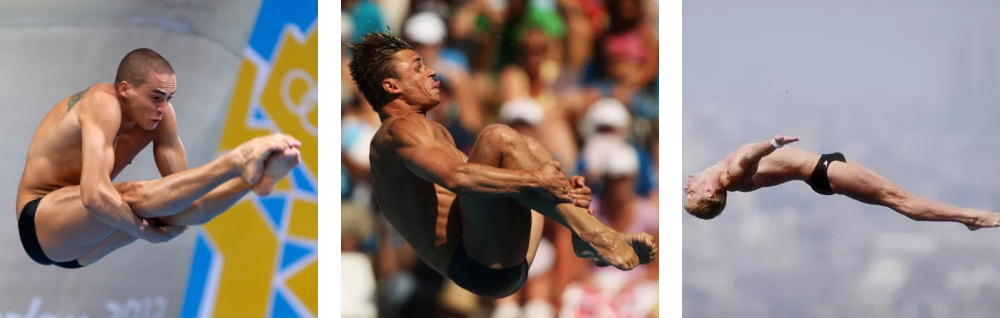
\includegraphics[scale=0.98]
{figures/dives.png}}
\caption{\label{fig:dive-styles} The figure shows the three main flight styles: pike, tuck, and straight respectively.}
\end{figure}

Our goal is to use spatio-temporal volumes to extract features that will then be used to train a convolutional neural network. This network will be used to classify previously unseen videos. Special importance will be placed in aggregating temporal data to solve possible short-term conflicts during the classification process, as the "pike" and "tuck" position can be confused for each other in certain angles. To train our network we plan to use the \textit{Diving48} dataset \cite{ref-diving48} which contains a large number of recordings from a variety of angles. All the videos in this dataset contain ground-truth labels that describe the sequence in four ways: (i) the type of takeoff, (ii) the number of somersaults, (iii) the number of twists, and (iv) the style of flight.

To simplify the extent of our work, we will remove the "free" flight style  from the dataset (i.e. the style where the performer combines several styles in one dive). Furthermore, we will clip the recordings to remove the parts where the performer sinks below the water. As a last preprocessing step, we will remove the performances with extreme camera angles. Afterwards, we will use the spatio-temporal volumes to extract features of interest (possibly legs and torso, as they can be easily segmented due to the separation provided by the swim trunk). Said features are represented as masks overlayed to the original video.

\section{Envisioned solution}

Lorem ipsum dolor sit amet, consetetur sadipscing elitr, sed diam nonumy eirmod tempor invidunt ut labore et dolore magna aliquyam erat, sed diam voluptua. At vero eos et accusam et justo duo dolores et ea rebum. Stet clita kasd gubergren, no sea takimata sanctus est Lorem ipsum dolor sit amet. Lorem ipsum dolor sit amet, consetetur sadipscing elitr, sed diam nonumy eirmod tempor invidunt ut labore et dolore magna aliquyam erat, sed diam voluptua. At vero eos et accusam et justo duo dolores et ea rebum. Stet clita kasd gubergren, no sea takimata sanctus est Lorem ipsum dolor sit amet.

Lorem ipsum dolor sit amet, consetetur sadipscing elitr, sed diam nonumy eirmod tempor invidunt ut labore et dolore magna aliquyam erat, sed diam voluptua. At vero eos et accusam et justo duo dolores et ea rebum. Stet clita kasd gubergren, no sea takimata sanctus est Lorem ipsum dolor sit amet. Lorem ipsum dolor sit amet, consetetur sadipscing elitr, sed diam nonumy eirmod tempor invidunt ut labore et dolore magna aliquyam erat, sed diam voluptua. At vero eos et accusam et justo duo dolores et ea rebum. Stet clita kasd gubergren, no sea takimata sanctus est Lorem ipsum dolor sit amet.

Lorem ipsum dolor sit amet, consetetur sadipscing elitr, sed diam nonumy eirmod tempor invidunt ut labore et dolore magna aliquyam erat, sed diam voluptua. At vero eos et accusam et justo duo dolores et ea rebum. Stet clita kasd gubergren, no sea takimata sanctus est Lorem ipsum dolor sit amet. Lorem ipsum dolor sit amet, consetetur sadipscing elitr, sed diam nonumy eirmod tempor invidunt ut labore et dolore magna aliquyam erat, sed diam voluptua. At vero eos et accusam et justo duo dolores et ea rebum. Stet clita kasd gubergren, no sea takimata sanctus est Lorem ipsum dolor sit amet.

\section{Expected results}

Lorem ipsum dolor sit amet, consetetur sadipscing elitr, sed diam nonumy eirmod tempor invidunt ut labore et dolore magna aliquyam erat, sed diam voluptua. At vero eos et accusam et justo duo dolores et ea rebum. Stet clita kasd gubergren, no sea takimata sanctus est Lorem ipsum dolor sit amet. Lorem ipsum dolor sit amet, consetetur sadipscing elitr, sed diam nonumy eirmod tempor invidunt ut labore et dolore magna aliquyam erat, sed diam voluptua. At vero eos et accusam et justo duo dolores et ea rebum. Stet clita kasd gubergren, no sea takimata sanctus est Lorem ipsum dolor sit amet.

\bibliography{references/references.bib}

\end{document}